\documentclass[conference]{IEEEtran}
\IEEEoverridecommandlockouts
% The preceding line is only needed to identify funding in the first footnote. If that is unneeded, please comment it out.
%Template version as of 6/27/2024

\usepackage{cite}
\usepackage{amsmath,amssymb,amsfonts}
\usepackage{algorithmic}
\usepackage{graphicx}
\usepackage{textcomp}
\usepackage{xcolor}
\def\BibTeX{{\rm B\kern-.05em{\sc i\kern-.025em b}\kern-.08em
    T\kern-.1667em\lower.7ex\hbox{E}\kern-.125emX}}
\begin{document}

\title{Rooting Out Atoms Of Confusion -- A Call To Action}

\author{\IEEEauthorblockN{Justin Cappos}
\IEEEauthorblockA{\textit{dept. name of organization (of Aff.)} \\
\textit{name of organization (of Aff.)}\\
City, Country \\
email address or ORCID}
\and
\IEEEauthorblockN{Dan Gopstein}
\IEEEauthorblockA{\textit{dept. name of organization (of Aff.)} \\
\textit{name of organization (of Aff.)}\\
City, Country \\
email address or ORCID}
\and
\IEEEauthorblockN{Renata Vaderna}
\IEEEauthorblockA{\textit{dept. name of organization (of Aff.)} \\
\textit{name of organization (of Aff.)}\\
City, Country \\
email address or ORCID}
\and
\IEEEauthorblockN{Yanyan Zhuang}
\IEEEauthorblockA{\textit{dept. name of organization (of Aff.)} \\
\textit{name of organization (of Aff.)}\\
City, Country \\
email address or ORCID}
}

\maketitle

\begin{abstract}
A few years ago, Gopstein et al. discovered that many bugs in software are 
caused by small, confusing patterns in code called Atoms of Confusion.  This 
finding has been replicated to different domains and validated in a variety of
ways, including brain wave scans with EEGs.   ...

We are a growing  community of academics which are bridging the industry / 
academic gap to put these ideas in practice.  We are currently adding data 
sharing and visualization tools, which are working with the Linux Foundation 
to host in a neutral, industry facing manner.  We 
have been working to deploy Atoms checking in the Linux Kernel and are also 
building a broader community through deep connections into large open source
ecosystems.  We invite you to join us!
\end{abstract}

\begin{IEEEkeywords}
component, formatting, style, styling, insert.
\end{IEEEkeywords}

\section{Introduction}

Software bugs represent a significant challenge worldwide, with a staggering cost of approximately \$2.08 trillion in the US alone in 2020, as reported by the Consortium for Information \& Software Quality (CISQ) \cite{CPSQ2020}. Addressing these bugs efficiently before they cause damage is crucial in both industry and academia.

Code review serves as a cornerstone of quality assurance in both open source and proprietary projects. Research highlights that inadequate code reviews are linked to diminished software quality, the emergence of anti-patterns, and increased post-release defects. Ensuring that software is understandable to humans is crucial yet challenging, often approached in an ad hoc manner.

Our research has delved into the causes of code confusion for human readers. We have identified and empirically validated small C code patterns, termed \emph{atoms of confusion}, which programmers often misinterpret. Analyzing 14 large C projects revealed hundreds of thousands of these atoms, highly correlated with both comments and bug fixes, underscoring their profound impact on software reliability \cite{gopstein2018prevalence}.

This body of work has inspired a breadth of subsequent studies across various programming languages, employing methodologies like eye-tracking and EEG to probe deeper into how programmers interact with these confusing elements \cite{langhout2021atoms, mendes2021bohr, mendes2022dazed, torres2023investigation, dacosta2023seeing, Manor2018AtomsConfusionSwift, yeh2017detecting}.

As this research started to gain momentum, we initiated efforts to enhance community collaboration. By fostering discussions, sharing datasets, and initiating research into unified standardization of what constitutes an atom of confusion, we aim to streamline the process for researchers to conduct future atoms-related experiments. Additionally, we are committed to expanding awareness and fostering interest in this novel approach of examining the causes of code confusion and bugs, not just within academia, but also across the industry.


\section{ Enhancing Community Engagement}


In our previous experience, organizing community meetings has proven to be an effective method for gathering individuals who are passionate about specific fields or projects. Since the beginning of this year, we have initiated bimonthly meetings to cultivate a strong sense of community among researchers interested in this field. During these gatherings, we encourage members to introduce themselves and to share both past and recent research. We ensure that lists of all published papers are readily accessible, and distribute notes and slides from presentations. Our primary aim is to establish a supportive platform where every participant can showcase their work and engage in constructive feedback exchanges within the community.

Furthermore, we've initiated discussions on challenges particularly relevant to those studying code confusion, such as conducting user studies. We hope that members of the community who are new to this area can learn from and seek guidance from experienced researchers who have conducted several user studies.

Another challenge we've tackled is the varied interpretations of what constitutes an atom of confusion. We've organized meetings specifically focused on this issue, presenting multiple code snippets that have been seen by some as atoms of confusion, while others may not find them confusing. These discussions have sparked significant interest and motivated further exploration into understanding these divisive elements.


\subsection{A Framework for Classifying Atoms of Confusion}

We have identified a core issue arising from the absence of a formal definition of what constitutes an atom of confusion. While our previous classifiers \cite{gopstein2018prevalence} have shown correlations between atoms of confusion, bugs, and confusing code, they have not succeeded in providing clear definitions. Our goal is to develop a precise, easily extendable, and reproducible methodology for classifying specific code patterns as atoms. To this end, we are actively developing a framework that includes mathematical guidelines to determine what is and isn't an atom. This framework is not only designed to support hypothesis testing among community members but also to pave the way for future applications to explore atoms in various programming languages. This effort builds upon our findings that increased frequencies of comments and bug fixes often indicate the presence of atoms, reinforcing their significant impact on software reliability.

The main idea behind this ongoing research is to count occurrences of all AST subtrees within large open source projects, as well as in bugfix commits and commented code snippets, looking for patterns with high frequencies of bugfixes and comments. The next step involves applying a formal statistical method (link to method here) to clearly distinguish atom candidates from non-atoms. This approach aims to provide a more precise and objective answer to questions about questionable patterns, potentially uncovering additional confusing patterns that were previously unrecognized. Additionally, researchers should be able to apply different metrics, adding new dimensions or substituting the measures of bugfix and comment frequencies.


\subsection{Collaboration with the Industry}

We aim for our research on atoms of confusion to surpass academic borders and have a tangible impact in the industry. Our previous research has led to the detection and fix of a bug in the Linux kernel caused by one of the patterns we consider to be an atom of confusion. This success demonstrates the potential for the practical impact of our work and highlights the importance of ongoing collaboration with industry.

The tool widely used to detect issues and refactor certain parts of the Linux kernel code is Coccinelle. Coccinelle is a program matching and transformation engine that provides the Semantic Patch Language (SmPL) for specifying desired matches and transformations in C code. It was initially designed to document and automate collateral evolutions in device driver code. Unlike traditional patches, which are limited to specific instances, Coccinelle's semantic patches can modify hundreds of files across thousands of code sites by abstracting away specific details and variations \cite{coccinelle}.

Given its extensive use, and in direct collaboration with the maintainers of Coccinelle, we are implementing the detection of atoms using Coccinelle. While our primary focus is on deployment within the Linux kernel, Coccinelle can be used to process any C code. Consequently, the semantic patches we have developed to detect atoms can also be applied to other C codebases. We have implemented patches for the detection of 14 out of 15 identified atoms, excluding only one that is beyond Coccinelle's capabilities. All these semantic patches are available in our GitHub repository \cite{githubcocci}. 

\subsection{Abbreviations and Acronyms}\label{AA}
Define abbreviations and acronyms the first time they are used in the text, 
even after they have been defined in the abstract. Abbreviations such as 
IEEE, SI, MKS, CGS, ac, dc, and rms do not have to be defined. Do not use 
abbreviations in the title or heads unless they are un

\subsection{Figures and Tables}\label{FAT}
\paragraph{Positioning Figures and Tables} Place figures and tables at the top and 
bottom of columns. Avoid placing them in the middle of columns. Large 
figures and tables may span across both columns. Figure captions should be 
below the figures; table heads should appear above the tables. Insert 
figures and tables after they are cited in the text. Use the abbreviation 
``Fig.~\ref{fig}'', even at the beginning of a sentence.

\begin{table}[htbp]
\caption{Table Type Styles}
\begin{center}
\begin{tabular}{|c|c|c|c|}
\hline
\textbf{Table}&\multicolumn{3}{|c|}{\textbf{Table Column Head}} \\
\cline{2-4} 
\textbf{Head} & \textbf{\textit{Table column subhead}}& \textbf{\textit{Subhead}}& \textbf{\textit{Subhead}} \\
\hline
copy& More table copy$^{\mathrm{a}}$& &  \\
\hline
\multicolumn{4}{l}{$^{\mathrm{a}}$Sample of a Table footnote.}
\end{tabular}
\label{tab1}
\end{center}
\end{table}

\begin{figure}[htbp]
\centerline{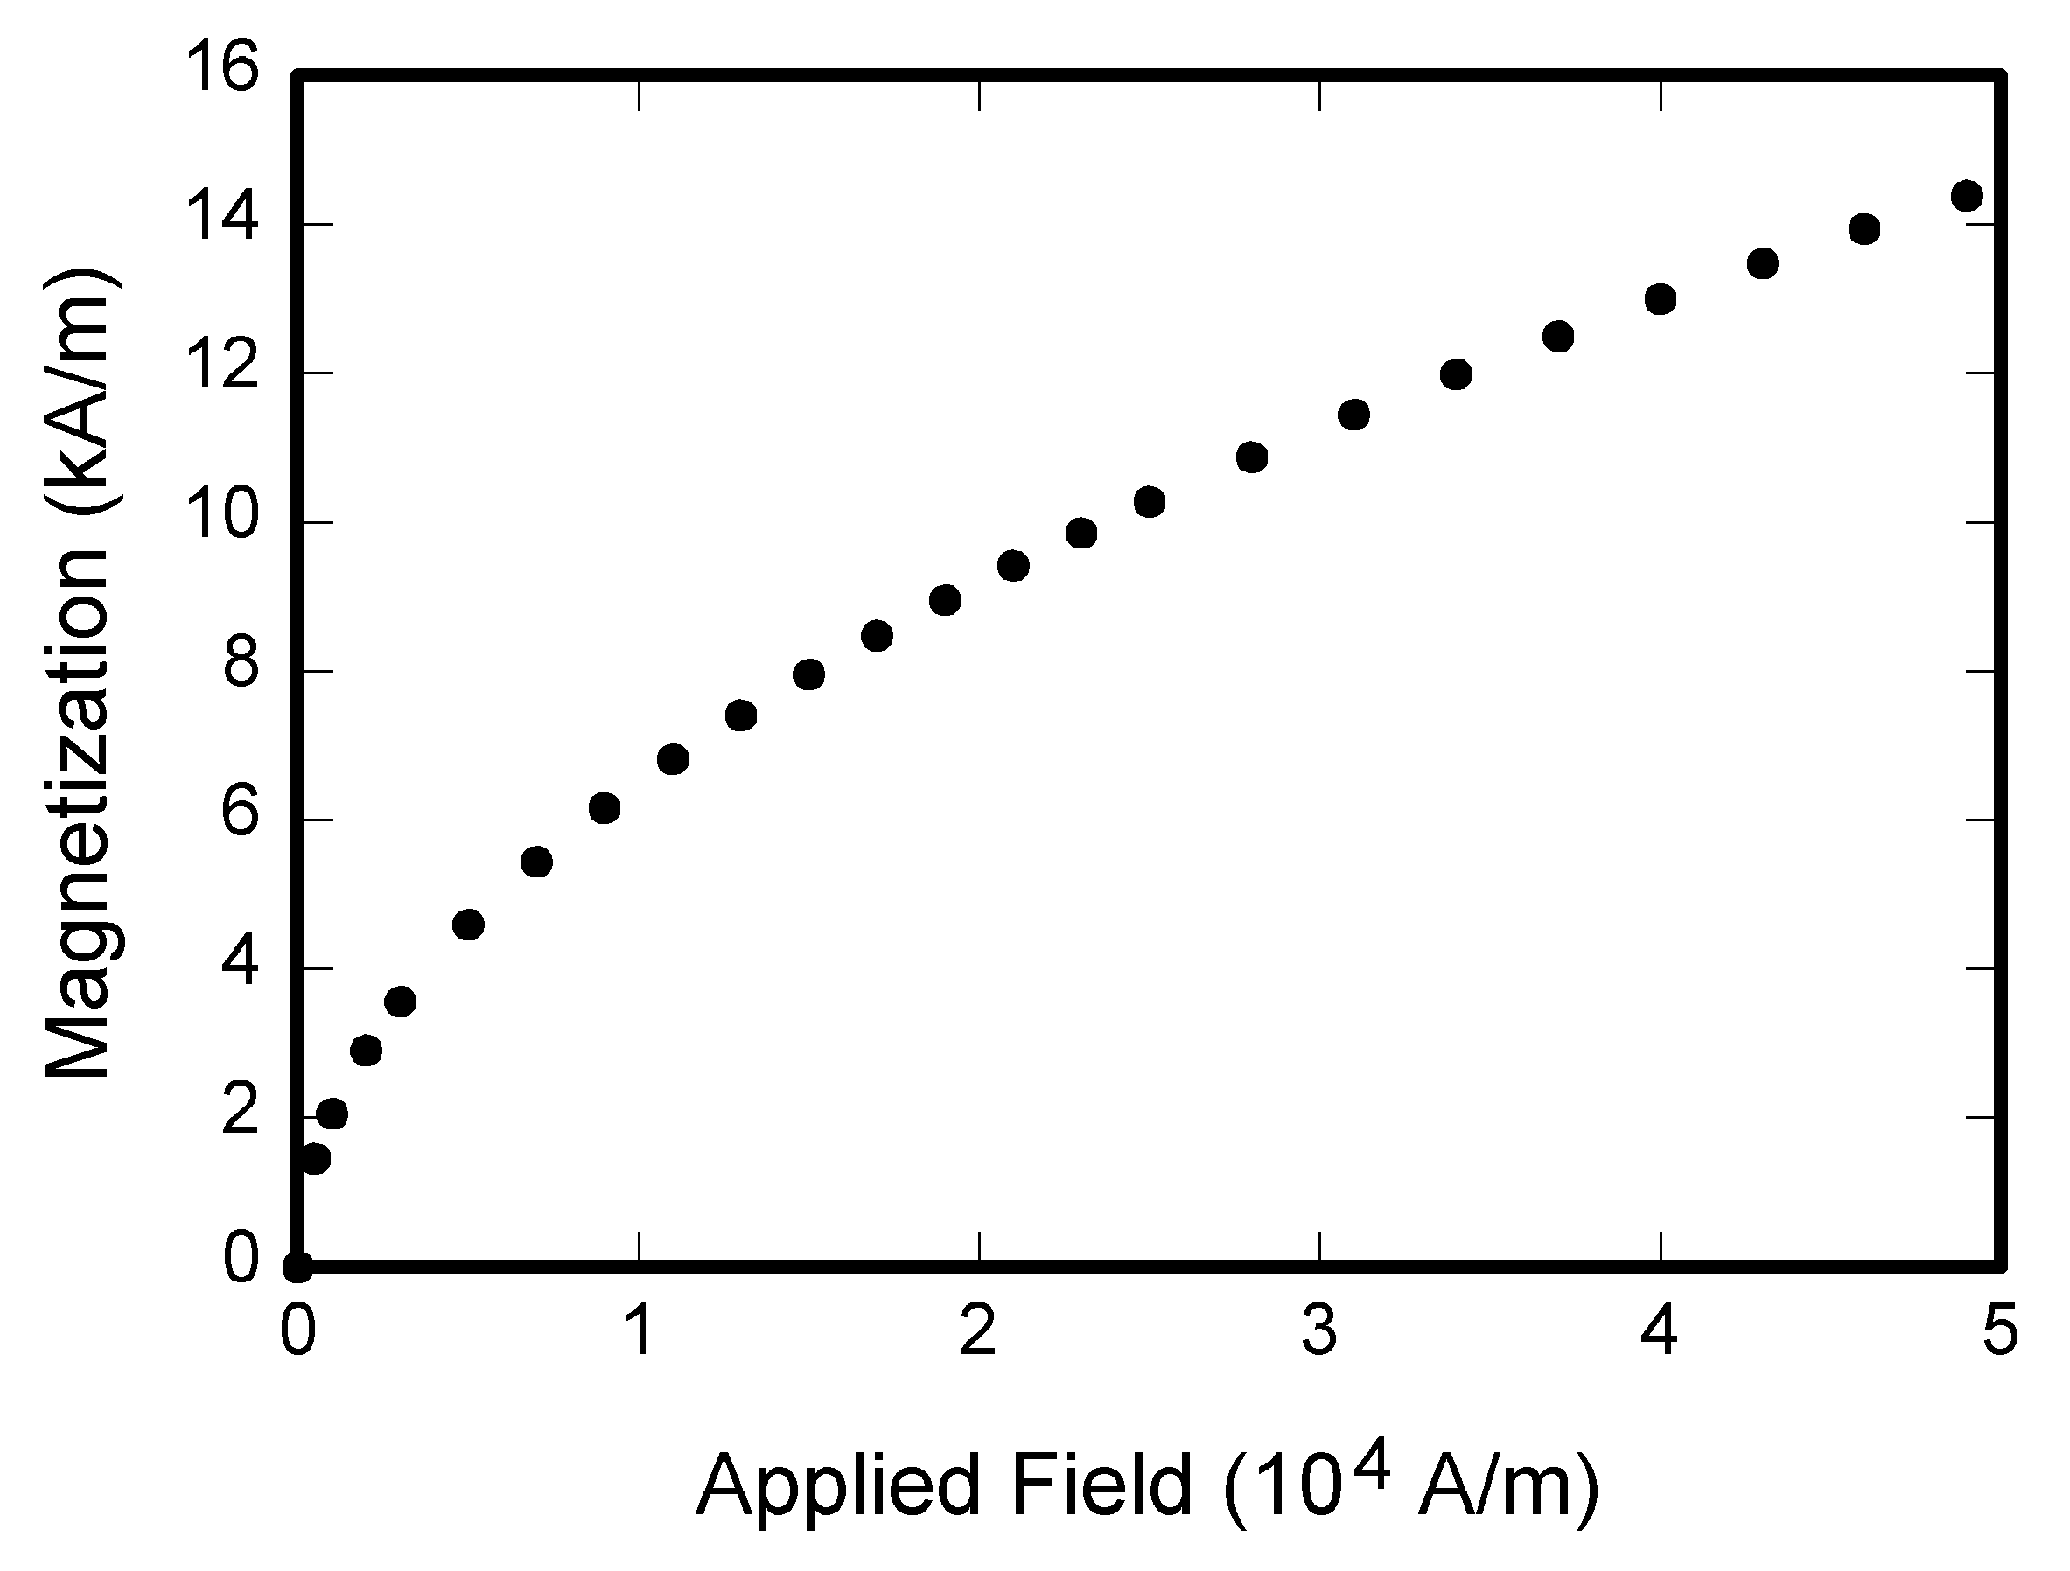
\includegraphics{fig1.png}}
\caption{Example of a figure caption.}
\label{fig}
\end{figure}

Figure Labels: Use 8 point Times New Roman for Figure labels. Use words 
rather than symbols or abbreviations when writing Figure axis labels to 
avoid confusing the reader. As an example, write the quantity 
``Magnetization'', or ``Magnetization, M'', not just ``M''. If including 
units in the label, present them within parentheses. Do not label axes only 
with units. In the example, write ``Magnetization (A/m)'' or ``Magnetization 
\{A[m(1)]\}'', not just ``A/m''. Do not label axes with a ratio of 
quantities and units. For example, write ``Temperature (K)'', not 
``Temperature/K''.

\section*{Acknowledgment}




\end{document}
